\documentclass{article}
\usepackage{graphicx}
\usepackage{alltt}
\usepackage{amsmath}
\usepackage{amsfonts}
\usepackage{bigstrut}
\usepackage{enumerate}
\usepackage{fancyhdr}
\usepackage[top=.75in, bottom=.95in, left=.75in, right=.75in]{geometry}
\usepackage{float}
\usepackage{lastpage}
\usepackage{tikz}
\usepackage[latin1]{inputenc}
\usepackage{color}
\usepackage{array}
\usepackage{longtable}
\usepackage{calc}
\usepackage{multirow}
\usepackage{hhline}
\usepackage{ifthen}
\usepackage{listings}
\usepackage{circuitikz}
\usepackage{tabto}
%\lstset{language=VHDL,basicstyle=\ttfamily}
\definecolor{mygreen}{rgb}{0,0.6,0}
\definecolor{mygray}{rgb}{0.5,0.5,0.5}
\definecolor{mymauve}{rgb}{0.58,0,0.82}
\lstset{ %
  backgroundcolor=\color{white},   % choose the background color; you must add \usepackage{color} or \usepackage{xcolor}; should come as last argument
  basicstyle=\normalsize,        % the size of the fonts that are used for the code
  breakatwhitespace=false,         % sets if automatic breaks should only happen at whitespace
  breaklines=true,                 % sets automatic line breaking
  captionpos=b,                    % sets the caption-position to bottom
  commentstyle=\color{mygreen},    % comment style
  deletekeywords={...},            % if you want to delete keywords from the given language
  escapeinside={\%*}{*)},          % if you want to add LaTeX within your code
  extendedchars=true,              % lets you use non-ASCII characters; for 8-bits encodings only, does not work with UTF-8
  frame=single,	                   % adds a frame around the code
  keepspaces=true,                 % keeps spaces in text, useful for keeping indentation of code (possibly needs columns=flexible)
  keywordstyle=\color{blue},       % keyword style
  language=VHDL,                   % the language of the code
  morekeywords={*,...},            % if you want to add more keywords to the set
  numbers=left,                    % where to put the line-numbers; possible values are (none, left, right)
  numbersep=5pt,                   % how far the line-numbers are from the code
  numberstyle=\tiny\color{mygray}, % the style that is used for the line-numbers
  rulecolor=\color{black},         % if not set, the frame-color may be changed on line-breaks within not-black text (e.g. comments (green here))
  showspaces=false,                % show spaces everywhere adding particular underscores; it overrides 'showstringspaces'
  showstringspaces=false,          % underline spaces within strings only
  showtabs=false,                  % show tabs within strings adding particular underscores
  stepnumber=2,                    % the step between two line-numbers. If it's 1, each line will be numbered
  stringstyle=\color{mymauve},     % string literal style
  tabsize=2,	                   % sets default tabsize to 2 spaces
  columns=flexible,
  breaklines=true,
  title=\lstname                   % show the filename of files included with \lstinputlisting; also try caption instead of title
}
\floatstyle{plain}
\restylefloat{figure}
\pagestyle{fancy}
\fancyhead{}
\fancyfoot{}
\setlength{\headheight}{59.0pt}
\def\inputGnumericTable{}
\fancyhead[CO]{\textbf{Air Force Institute of Technology\\Department of Electrical and Computer Engineering\\
Cryptography and Data Security (CSCE 544)}\\ Homework \#2\\
 Micah Hayden}
\lhead{\today}
\rhead{Page \thepage{} of \pageref{LastPage} }
\newlength\tindent
\setlength{\tindent}{\parindent}
\setlength{\parindent}{0pt}
\renewcommand{\indent}{\hspace*{\tindent}}

\usepackage[style=numeric, sorting=none]{biblatex}
\bibliography{myreferences.bib}

\begin{document}
    \section*{[100 Points] Implement the encryption and decryption functions in Python for an Affine Cipher that takes as input the corresponding ciphertext/plaintext, and  arbitrary alphabet $A$ such that  $26 \leq |A| \leq 256$. Make sure that the cipher implementation warns users about invalid inputs.}

My Python implementation for this is shown in Appendix A.

    \section*{[40 Points] Consider an unfair coin where the two outcomes, heads and tails have probabilities $p(\textit{heads})=p$ and $p(\textit{tails})=1-p$}
    \begin{enumerate}
      \item [(a)] If the coin is flipped two times, what are the possible outcomes along with their respective probabilities?
      
      \item HH, $p(HH) = p^2$
      \item HT, $p(HT) = p \cdot (1-p)$
      \item TH, $P(TH) = (1-p) \cdot p$
      \item TT, $p(TT) = (1-p)^2$
      
      \item [(b)] Show that the entropy in part (a) is $-2p\log_2(p)-2(1-p)\log_{2}(1-p)$. How could this have been predicted without calculating probabilites in part (a)?
      
      One can calculate the entropy using Shannon's Entropy, which is Equation \ref{eq:Entropy} below.
      
      \begin{equation}
      \label{eq:Entropy}
      H(X) = - \sum_{x \in X} p(x) \cdot \log_2 p(x)
      \end{equation}

For our case, there are four possibilities, with the probabilities shown above.
	\begin{align*}
	H(X) = - p^2 \cdot \log_2 p^2 - 2 \cdot p \cdot (1-p) \cdot \log_2 [p \cdot (1-p)] - (1-p)^2 \cdot \log_2 (1-p)^2 \\
	\end{align*}
This can be expanded by using the properties of exponents to simplify into the expected expression, as shown below:
\begin{align*}
H(X) &= -2  p^2 \log_2 p - 2  p  (1-p)  \log_2 p - 2  p  (1-p) \log_2 (1-p) - 2  (1-p)^2  \log_2 (1-p) \\
\end{align*}
Now group by $\log_2p$ and $\log_2(1-p)$:

\begin{minipage}{.5\textwidth}
\begin{align*}
\text{Terms for} \log_2p:  \\ \hline
-2p^2\log_2 p -2p \log_2p + 2p^2\log_2p \\
 = -2 p \log_2p \\  
 \\
\end{align*}
\end{minipage}
\begin{minipage}{.5\textwidth}
\begin{align*}
\text{Terms for} \log_2(1-p): \\ \hline
-2p\log_2(1-p) +2p^2\log_2(1-p)-2\log_2(1-p)+ \dots \\
+ 4p\log_2(1-p)-2p^2\log_2(1-p) \\
= (2p-2) \cdot \log_2(1-p) \\
= -2 \cdot (1-p) \cdot \log_2(1-p)
\end{align*}
\end{minipage}
The sum of the two terms above are the expression for entropy:
$$ H(X) = -2  p  \log_2p - 2  (1-p)  \log_2(1-p) $$

This value could be predicted by assuming the worst case entropy:  $p(heads) = p(tails)$.
This leads to the following expression for entropy:  $H(X) = log_2|A|$, where $|A|$ is the number of possible outcomes.
For 2 coin flips, the maximum entropy would be $H(X) = log_2 4 = 2$.
    \end{enumerate}

    \section*{[60 Points] Decipher the following ciphertext using ciphertext-only cryptanalysis. Note the alphabet used to create is this ciphertext is as following: [abcdefghijklmnopqrstuvwxyz]}

    \subsection*{[30 Points] Ciphertext \#1 (Affine)}
    \begin{verbatim}
        azwcwlugblyciuohxfoxaiallcsrrwhxobzzupubzxfuewbcxaxsxawbwpxfusbaxu
        zcxoxucokoabcxollubugaucpwhuakbobzzwgucxaexfoxaialljuohxhsupoaxfob
        zollukaobeuxwxfucoguxfoxaxoquxfacwjlakoxawbphuulyiaxfwsxobygubxolh
        ucuhnoxawbwhrshrwcuwpunocawbobzxfoxaialliullobzpoaxfpsllyzacefohkux
        fuzsxaucwpxfuwppaeuwbifaefaogojwsxxwubxuhcwfulrguk
    \end{verbatim}

I decrypted this ciphertext using a brute force attack, determining the key is $\alpha = 21$, $\beta = 14$, producing the below output:

\begin{figure}[h!]
\centering
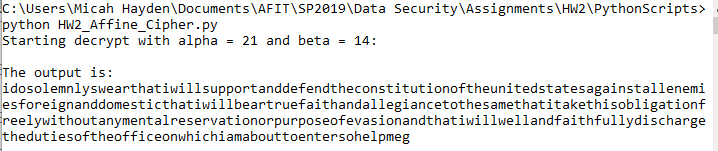
\includegraphics[scale=1.0]{Images/run_Affine.PNG}
\caption{Output of my Affine python script with $\alpha = 21$, $\beta = 14$}
\label{fig:affineOut}
\end{figure}

    \subsection*{[20 Points] Ciphertext \#2 (Vigen\`{e}re)}
    \begin{verbatim}
        kvqkqdgepdakywcjvzclkokdnkwhrgtlcffvgxgffljwegpkvavmvaqfqxvzgmpavwfkvsvwus
        iskfulcdnwpwoagkhgtwkypspvfgowulkuvzclkokdntgstltmgxcavzcffsndgykspuglqljwuso
        wcffljsvayandqtgqvzggtvgjughljwrjgkkvgfvghljwwfklgvulclgkcffljwqjfwtkqxvzgghxku
        gjusrhqaplgvqngjowcuegtvkfilqjgywdclkgpkcffljwwfkxqjouqvgghekdklcjabwkvaewugj
        wnhowigf
    \end{verbatim}

I utilized the vigenereHacker.py script described in \cite{CrackingCodes} to determine the likely key to the ciphertext, with the output shown below:

\begin{figure}[h!]
\centering
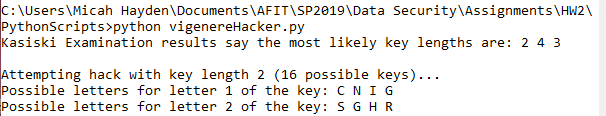
\includegraphics[scale=1.0]{Images/run_HackVig_1.PNG}
\caption{Likely keys of given ciphertext}
\label{fig:vigOut_1}
\end{figure}

\newpage
I then utilized an online vigenere cipher decoder \cite{Web}, with the first likely key \textbf{"cs"}.
This produced the following plaintext:
	\begin{verbatim}
		idosolemnlyswearthatiwillsupportanddefendtheconstitutionoftheunitedstatesa
        gainstallenemiesforeignanddomesticthatiwillbeartruefaithandallegiancetothesam
        eandthatiwillobeytheordersofthepresidentoftheunitedstatesandtheordersoftheoffic
        ersappointedovermeaccordingtoregulationsandtheuniformcodeofmilitaryjusticesoh
        elpmegod
	\end{verbatim}
	
    \subsection*{[10 Points] Ciphertext\#3 (Vigen\`{e}re)}
    
    \begin{verbatim}
        ujltkvbpxowvvcoqcubiubrkjofvtlpwvbuwplxtvkpytvkflnbzqxdcqgkqeqxuykbvlturvpxtw
        dmcepwwjvlunrpmvtqrsflocuzcqerobkqujduarvyrvngujlomqpvkjpjxcvxtroizjvkjvlohddv
        qpvkjpjjuzsqqhylujlukwjukjikmaxowvvcoujrviktvxealucqevkjpnbdrvvludxuarvuwjnonc
        boqwgkqecqzvkjpjpfgcwwjhbpwzptnbvlucejvbpwpjikuhlofrvvwsawpfrtqzjvkpwwbpbdq
        ddjloi
    \end{verbatim}

To crack this ciphertext, I utilized the same sequence and resources \cite{CrackingCodes} and \cite{Web}.
\begin{figure}[h!]
\centering
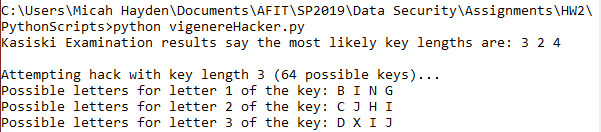
\includegraphics[scale=1.0]{Images/run_HackVig_2.PNG}
\caption{Likely keys of given ciphertext}
\label{fig:vigOut_2}
\end{figure}

I attempted the first likely key, \textbf{"bcd"}, which produced the below plaintext:
	\begin{verbatim}
        thisisanunusualparagraphimcuriousastojusthowquicklyyoucanfindoutwhatissounusu
        alaboutititlookssoordinaryandplainthatyouwouldthinknothingwaswrongwithitinfact
        nothingiswrongwithititishighlyunusualthoughstudyitandthinkaboutitbutyoustillma
        ynotfindanythingoddbutifyouworkatitabityoumightfindouttrytodosowithoutanyco
        aching
	\end{verbatim}
The "unusual" aspect of the plaintext is that there are no occurrences of the letter "e".

\printbibliography

\newpage
\section*{Appendix A:  Python Script for Affine Cipher}
\lstinputlisting[language=Python]{PythonScripts/HW2_Affine_Cipher.py}

\end{document}
